\documentclass[12pt]{article}
\usepackage[top=1in,left=1in, right = 1in, footskip=1in]{geometry}

\usepackage{graphicx}
\usepackage{xspace}
%\usepackage{adjustbox}

\newcommand{\comment}{\showcomment}
%% \newcommand{\comment}{\nocomment}

\newcommand{\showcomment}[3]{\textcolor{#1}{\textbf{[#2: }\textsl{#3}\textbf{]}}}
\newcommand{\nocomment}[3]{}

\newcommand{\jd}[1]{\comment{cyan}{JD}{#1}}
\newcommand{\swp}[1]{\comment{magenta}{SWP}{#1}}
\newcommand{\bmb}[1]{\comment{blue}{BMB}{#1}}
\newcommand{\djde}[1]{\comment{red}{DJDE}{#1}}

\newcommand{\eref}[1]{Eq.~\ref{eq:#1}}
\newcommand{\fref}[1]{Fig.~\ref{fig:#1}}
\newcommand{\Fref}[1]{Fig.~\ref{fig:#1}}
\newcommand{\sref}[1]{Sec.~\ref{#1}}
\newcommand{\frange}[2]{Fig.~\ref{fig:#1}--\ref{fig:#2}}
\newcommand{\tref}[1]{Table~\ref{tab:#1}}
\newcommand{\tlab}[1]{\label{tab:#1}}
\newcommand{\seminar}{SE\mbox{$^m$}I\mbox{$^n$}R}

\usepackage{amsthm}
\usepackage{amsmath}
\usepackage{amssymb}
\usepackage{amsfonts}

\usepackage{lineno}
\linenumbers

\usepackage[pdfencoding=auto, psdextra]{hyperref}

\usepackage{natbib}
\bibliographystyle{chicago}
\date{\today}

\usepackage{xspace}
\newcommand*{\ie}{i.e.\@\xspace}

\usepackage{color}

\newcommand{\Rx}[1]{\ensuremath{{\mathcal R}_{#1}}\xspace} 
\newcommand{\Ro}{\Rx{0}}
\newcommand{\Rc}{\Rx{\mathrm{c}}}
\newcommand{\RR}{\ensuremath{{\mathcal R}}\xspace}
\newcommand{\Rhat}{\ensuremath{{\hat\RR}}}
\newcommand{\Rintrinsic}{\ensuremath{{\mathcal R}_{\textrm{\tiny intrinsic}}}\xspace}
\newcommand{\tsub}[2]{#1_{{\textrm{\tiny #2}}}}
\newcommand{\dd}[1]{\ensuremath{\, \mathrm{d}#1}}
\newcommand{\dtau}{\dd{\tau}}
\newcommand{\dx}{\dd{x}}
\newcommand{\dsigma}{\dd{\sigma}}

\newcommand{\pt}{p} %% primary time
\newcommand{\st}{s} %% secondary time

\newcommand{\psize}{{\mathcal P}} %% primary cohort size
\newcommand{\ssize}{{\mathcal S}} %% secondary cohort size

\newcommand{\gtime}{\sigma} %% generation interval
\newcommand{\gdist}{g} %% generation-interval distribution

\newcommand{\total}{{\mathcal T}} %% total number of serial intervals

\begin{document}

\begin{flushleft}{
	\Large
	\textbf\newline{
		Unraveling the paradox between generation and serial intervals
	}
}
\newline
\\
Sang Woo Park\textsuperscript{1,*}
Kaiyuan Sun\textsuperscript{2}
Benjamin M.\ Bolker\textsuperscript{3,4,5}
David Champredon\textsuperscript{6}
David J.\,D.\ Earn\textsuperscript{4,5}
Michael Li\textsuperscript{3}
Joshua S.\ Weitz\textsuperscript{7, 8}
Bryan T.\ Grenfell\textsuperscript{1,2,9}
Jonathan Dushoff\textsuperscript{3,4,5,*}
\\
\bigskip
\textbf{1} Department of Ecology and Evolutionary Biology, Princeton University, Princeton, NJ, USA
\\
\textbf{2} Fogarty International Center, National Institutes of Health, Bethesda, MD, USA
\\
\textbf{3} Department of Biology, McMaster University, Hamilton, ON, Canada
\\
\textbf{4} Department of Mathematics and Statistics, McMaster University, Hamilton, ON, Canada
\\
\textbf{5} M.\,G.\,DeGroote Institute for Infectious Disease Research, McMaster University, Hamilton, ON, Canada
\\
\textbf{6} Department of Pathology and Laboratory Medicine, University of Western Ontario, London, Ontario, Canada
\\
\textbf{7} School of Biological Sciences, Georgia Institute of Technology, Atlanta, GA, USA
\\
\textbf{8} School of Physics, Georgia Institute of Technology, Atlanta, GA, USA
\\
\textbf{9} Woodrow Wilson School of Public and International Affairs, Princeton University, Princeton, NJ, USA
\\
\bigskip

*Corresponding author: swp2@princeton.edu
\end{flushleft}

\section*{Abstract}

Generation and serial intervals are under-appreciated --- often treated as auxiliary variables for estimating the reproduction number \RR --- yet important quantities for charaterizing the outset of an outbreak.
Even though their differences were clearly laid out over a decade ago, there is still a need for clear conceptual and theoretical understanding of their roles in shaping the epidemiological dynamics.
A part of the confusion can be attributed to an apparent paradox.
By definition, both generation and serial intervals describe how infection spreads between individuals, and therefore, one would expect them to potentially provide the same link between the epidemic growth rate $r$ and the reproduction number \RR.
However, current theory does not explain how two different distributions can give the same link between $r$ and \RR --- some studies have further demonstrated that generation and serial intervals give different $r$--\RR link.
We provide an answer to the paradox by showing that if serial intervals are defined as \emph{forward-looking} intervals during the exponential phase, then the correct link between $r$ and \RR emerges.
We also provide a heuristic way of addressing potential biases that can arise from not accounting for changes in these references and apply our framework to serial intervals of COVID-19.
Our study demonstrates the importance of early epidemiological investigation through contact tracing for characterizing initial serial intervals and further provides rationale for reassessing serial intervals of COVID-19.

\pagebreak

\section{Introduction}

The reproduction number \RR is one of the most important characteristics of an emerging epidemic such as novel coronavirus disease (COVID-19) \citep{majumder2020early}.
The reproduction number is defined as the average number of secondary cases caused by a primary case;
the corresponding reproduction number in a fully susceptible population --- referred to as the basic reproduction number \Ro --- allows us to predict the extent to which a disease will spread in the population and the amount of intervention to prevent an outbreak \citep{anderson1991infectious}.
Since reproduction number cannot be measured directly, particularly during the outset of an outbreak, it is often estimated from the observed exponential growth rate using generation- and serial-interval distributions (e.g., \cite{du2020serial, jung2020real, li2020early, zhao2020preliminary}).

The generation interval is defined as the time between when an individual (infector) is infected and when an individual infects another person (infectee);
the generation-interval distribution determines the relationship between the exponential growth rate $r$ and the reproduction number \RR \citep{wallinga2007generation}.
Similarly, the serial interval is defined as the time between when an infector and an infectee become \emph{symptomatic} \citep{svensson2007note}.
While serial intervals are similar to generation intervals, previous studies have noted that, in many contexts, serial intervals are expected to have larger variances than generation intervals but have the same mean \citep{svensson2007note,klinkenberg2011correlation,te2013estimating,champredon2018equivalence};
some studies further suggested that using serial intervals can give different estimates of \RR \citep{britton2019estimation}.

Although these distributions were clearly distinguished over a decade ago \citep{svensson2007note}, 
the need for a better conceptual and theoretical framework for understanding their differences is becoming clearer as the COVID-19 pandemic unfolds.
Researchers continue to rely on both generation and serial intervals to make inferences about COVID-19, particularly for estimating its \RR, without making a clear distinction \citep{tempvar,du2020serial,he2020temporal,wu2020nowcasting,zhao2020serial}.
Some studies still refer to time between infection (i.e., generation intervals) as serial intervals \citep{anderson2020will,hellewell2020feasibility}.

One important source of confusion comes down to an apparent paradox.
When the epidemic is growing exponentially, the spread of infection can be characterized as a ``renewal process'' based on previous incidence of infection, the associated generation-interval distribution, and the average infectiousness of an infected individual.
This renewal formulation allows us to link the exponential growth rate of an epidemic $r$ with its reproduction number \RR using the generation-interval distribution \citep{wallinga2007generation}.
By definition, the serial-interval distribution describes the renewal process between symptomatic cases based on their symptom onset dates;
therefore, both generation- and serial-interval distributions should potentially give us identical estimates of  \RR based the observed epidemic growth rate $r$.
In contexts where the distributions are expected to be different, current theory has no explanation for how they might provide identical estimates of \RR from $r$ (cf. \cite{britton2019estimation}).

Here, we provide an answer to this paradox, by showing that the relevant interval for the renewal framework is what is called the ``forward'' interval, and that the forward serial (but not generation) interval is affected by the rate of growth $r$ during the exponential-growth phase.
We develop a new framework for understanding serial intervals and show that the initial forward serial-interval distribution correctly links $r$ and \RR.
%\jd{Come back to this. Not just over time, right?} \swp{What do you mean? Everything is about time here... you haven't read the results section so maybe that's why?}
However, using inaccurately defined serial intervals or failing to account for changes in the observed serial-interval distributions over the course of an epidemic can bias the estimate of \RR, as inferred from the observed growth rate $r$.
We apply our framework to serial intervals of COVID-19 and lay out several principles to consider in using information about serial intervals and other epidemiological time delays in the analysis of the ongoing pandemic.

\section{Methods}

\subsection{Forward and backward delay distributions}

We first begin by describing a general framework for characterizing a distribution of time delays between two epidemiological events;
these events can be defined either within an infected individual (e.g., infection and symptom onset of an individual, the incubation period) or between infected individuals (e.g., symptom onsets of an infector and an infectee, the serial interval).
We can further divide these events into \emph{primary} and \emph{secondary} events.
When we measure an epidemiological time delay within an infected individual (e.g., the incubation period), the primary event is the event that always or usually occurs before the secondary event ---
most epidemiological events that can be observed within an individual have clear direction (e.g., infection and onset of symptoms) but some may not (e.g., onset of infectiousness and onset of symptoms).
% \jd{Rethink, or else rethink ``any'' above: the ``hidden'' time (my term) is the time between onset of infectiousness and onset of symptoms; it is within, but can be positive or negative. I'm not saying we should use it here\ldots}
When we measure an epidemiological time delay between infected individuals (e.g., the serial interval), 
the primary and secondary events are defined in terms of the direction of transmission:
The primary event refers to the event that occurs within the infector
and does not necessarily occur before the secondary event (which
occurs within the infectee).

We model time delays between a primary and a secondary event from a cohort perspective.
A primary cohort consists of \emph{all} individuals whose primary event occurred at a given time; 
a secondary cohort is defined similarly based on the secondary events.
For example, when we are measuring incubation periods, a \textbf{p}rimary cohort at time $\pt$ consists of all infected individuals who became infected at time $\pt$. 
Similarly, when we are measuring serial intervals, a primary cohort at time $\pt$ consists of all infectors who became symptomatic at time $\pt$.
Then, for each primary cohort $\pt$, we can define the expected time distribution between primary and secondary events.
We refer to this distribution as the forward delay distribution and denote it as $f_\pt(\tau)$.

Likewise, we define the backward delay distribution $b_\st(\tau)$ for a \textbf{s}econdary cohort at time $\st$:
The backward delay distribution describes the time delays between a primary and secondary host given that the secondary event occurred at time $\st$.
For example, the backward incubation period distribution at time $\st$ describes incubation periods for a \emph{cohort} of individuals who became symptomatic at time $\st$.
Likewise, the backward serial-interval distribution at time $\st$ describes serial intervals for a \emph{cohort} of infectees who became symptomatic at time $\st$.

At the individual level, both forward and backward \emph{perspectives}
must yield identical results (e.g., the length of the incubation
period of a given individual is the same whether measured forward from
the time of infection or backward from the time of symptom onset).
Consequently, if we restrict attention to individuals with a given
incubation period, say $\tau$, and we count how many became infected at time $\pt$
or how many first showed symptoms at time $\st=\pt+\tau$ then we must obtain
the same number. In general, no matter how delays are distributed, if
$\mathcal P$ and $\mathcal S$ represent the sizes of primary and
secondary cohorts then we must have
\begin{equation}
\psize(\pt) f_\pt(\tau) = \ssize(\st) b_\st(\tau) \,.
\label{eq:match}
\end{equation}
Substituting $\pt=\st-\tau$, it follows that
\begin{equation}
b_\st(\tau)= \frac{\psize(\st-\tau) f_{\st-\tau} (\tau)}{\ssize(\st)}
\label{eq:backward}
\end{equation}
If we are thinking of incubation periods, then the left hand side of
this equation is the probability density that there is an individual
who became symptomatic at time $\st$ after an incubation period of
length $\tau$. From the right hand side, we see that this probability
density depends on how many individuals became infected at time
$\st-\tau$ [$\psize(\st-\tau)$], how many individuals became
symptomatic at time $\st$ [$\ssize(\st)$], and the probability density
that someone who was infected at time $\st-\tau$ became symptomatic at
time $\st$ [$f_{\st-\tau}(\tau)$]. In general, Eq.~\eqref{eq:backward}
shows that the the backward delay distribution at reference time $\st$
[$b_\st(\tau)$] depends not only on the secondary cohort size at time
$\st$ [$\ssize(\st)$], but also on the primary cohort size at the
earlier time $\st-\tau$ [$\psize(\st-\tau)$] and the forward delay
distribution at that earlier time [$f_{\st-\tau}(\tau)$].

There are multiple mechanisms that drive the changes in forward and backward delay distributions over time ---
we begin by describing factors that affect the forward delay distributions.
Typically, within-individual forward delay distributions that reflect life history of a disease is expected to remain invariant over the course of an epidemic; 
these distributions include incubation period distribution.
Within-individual forward delay distributions that depend on external interventions, such as time distribution of symptom onset to hospitalization, can change over the course of an epidemic.
Between-individual forward delay distributions, such as generation- or serial-interval distributions, depend on epidemic dynamics;
for example, the forward generation intervals to contract during the outbreak because infected individuals are less likely to infect others later due to susceptible depletion \citep{champredon2015intrinsic}.

Changes in the backward delay distributions are affected by the changes in the forward delay distributions as it is evident from \eref{backward}.
Backward delay distributions also depend on changes in the primary cohort size over time due to conditionality of observations: 
The backward delay distribution is measured for a cohort of individuals whose secondary events occurred at the same time.
When the cohort size is increasing (or decreasing) over time, we are biased to observe shorter (or longer) delays when we look backward.
In particular, when the incidence is growing exponentially, we can calculate the amount of bias exactly.
Assuming that the forward delay distribution remains constant during the exponential growth phase ($\tsub{f}{exp}$), we have:
\begin{equation}
\tsub{b}{exp}(\tau) \propto \exp(-r\tau) \tsub{f}{exp}(\tau),
\label{eq:backexp}
\end{equation}
where $r$ is the exponential growth rate.
For faster epidemic (higher $r$), the backward delay distributions will be shorter.
Therefore, the backward delay distributions will be generally different from the forward delay distributions even if we are measuring time delays that are intrinsic to life history of a disease (e.g., incubation period).
These ideas apply to all epidemiological delay distributions and generalize the work by \cite{champredon2015intrinsic} who compared forward and backward generation-interval distributions to describe the realized generation intervals from the perspective of an infector and an infectee, respectively, as well as the work by \cite{britton2019estimation} who showed that \eref{backexp} holds for the backward generation-interval distributions.

\subsection{Realized serial interval distributions}

The serial interval is defined as the time between when an infector becomes symptomatic and when and infectee becomes symptomatic \citep{svensson2007note}.
Previous studies have often expressed serial intervals $\tau$ in the form (\fref{diagram}A):
\begin{equation}
\tau = (\gtime + x_1) - x_0
\end{equation}
where $x_0$ and $x_1$ represent the realized time from infection to symptom onset of an infector and an infectee, respectively, and $\gtime$ represents the realized generation interval.
These studies assumed that $x_0$ and $x_1$ follow the same distributions and concluded that the serial and generation intervals have the same mean \citep{svensson2007note,klinkenberg2011correlation,champredon2018equivalence, britton2019estimation};
however, this conclusion is based on the implicit assumption that serial intervals are measured from the perspective of a cohort of infectors that share the same infection time.
We refer to this definition as the intrinsic serial interval.

\begin{figure}[!th]
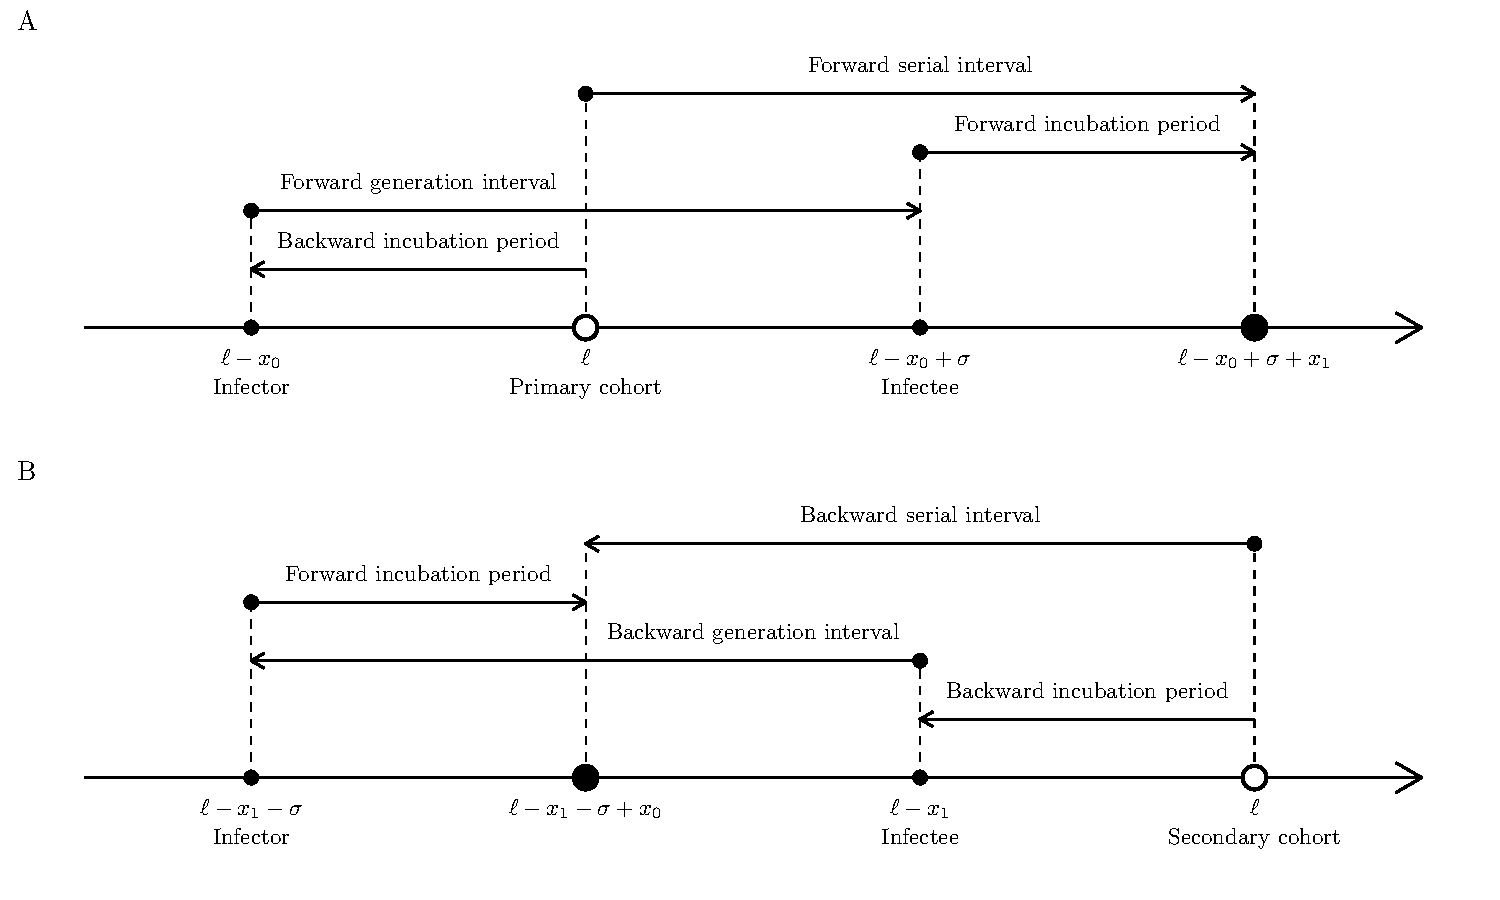
\includegraphics[width=\textwidth]{serial_guide.pdf}
\caption{
\textbf{Illustration of intrinsic, forward and backward serial intervals.}
(A) The intrinsic serial interval for a cohort of individuals infected at time $\pt$.
In this case, $x_0$ follows the forward incubation period distribution;
$\gtime$ follows the forward generation-interval distribution;
and $x_1$ follows the forward incubation period distribution.
(B) The forward serial interval for a cohort of infectors who became symptomatic at time $\pt$.
In this case, $x_0$ follows the backward incubation period distribution;
$\gtime$ follows the forward generation-interval distribution;
and $x_1$ follows the forward incubation period distribution.
(C) The backward serial interval for a cohort of infectees who became symptomatic at time $\st$.
In this case, $x_0$ follows the forward incubation period distribution;
$\gtime$ follows the backward generation-interval distribution;
and $x_1$ follows the backward incubation period distribution.
}
\label{fig:diagram}
\end{figure}

Since serial intervals describe the renewal process between symptomatic cases based on their symptom onset dates, we have to define serial intervals from the perspective of a cohort (of either infectors or infectees) of individuals that share the same symptom onset time.
The cohort-based framework allows us to understand the distribution of serial intervals we expect to observe when incidence is changing.
Given that an infector became symptomatic at time $\pt$, we first go backward in time by asking when the infector was infected, and then go forward in time by asking first when the infectee was infected and then when the infectee became symptomatic;
this defines the forward serial interval.
In \fref{diagram}B, we see that $x_0$ follows the backward incubation period distribution of the cohort of infectors who became symptomatic at time $\pt$;
$\gtime$ follows the forward generation-interval distribution of the cohort of infector who came infected at time $\pt - x_0$;
and $x_1$ follows the forward incubation period distribution of the cohort of infectees who became infected at time $\pt - x_0 + \gtime$.

Likewise, we can define the backward serial interval distribution for a secondary cohort $\st$ (\fref{diagram}C).
Given that an infectee became symptomatic at time $\st$, we have to first go backward in time by asking when the infectee became infected and when the infector became infected; 
then, we have to go forward in time by asking when the infector became symptomatic.
In this case, $x_1$ follows the backward incubation period distribution of the cohort of infectees who became symptomatic at time $\st$;
$\gtime$ follows the backward generation-interval distribution of the cohort of infectees who became infected at time $\st-x_1$;
and $x_0$ follows the forward incubation period distribution of the cohort of infectors who became infected at time $\st-x_1-\gtime$.
This conceptual framework clearly demonstrates that the distributions of $x_0$, $\st$, and $x_1$ (and therefore the distributions of serial intervals) depend on the reference cohort and the corresponding cohort time.

In order to define forward and backward serial interval distributions, we begin by modeling the total number of serial intervals $\total(\pt,\st)$ between time $\pt$ and $\st$ (i.e., total number of infection in which infectors develop symptom at time $\pt$ and infectees develop symptom at time $\st$).
The number of serial intervals between time $\pt$ and $\st$ given that the infectors became infected at time $\alpha_1$ and the infectees became infected at time $\alpha_2$ is can be then expressed as a product of (i) incidence $i$ at time $\alpha_1$, (ii) their case reproduction number $\Rc(\alpha_1)$ (i.e., the average number of secondary cases caused by a primary case infected at time $\alpha_1$ over the course of their infection, \cite{fraser2007estimating}), (iii) the density of forward generation interval between $\alpha_1$ and $\alpha_2$, and (iv) the densities of forward incubation periods between $\alpha_1$ and $\pt$ (incubation periods of infectors) as well as $\alpha_2$ and $\st$ (incubation periods of infectees):
\begin{equation}
\underbrace{\Rc (\alpha_1)}_{\substack{\text{case} \\ \text{reproduction} \\ \text{number}}} 
\times 
\underbrace{i(\alpha_1)}_{\text{incidence}} 
\times 
\underbrace{h_{\alpha_1}(\pt-\alpha_1, \alpha_2 - \alpha_1)}_{\substack{\text{joint density of} \\ \text{the forward incubation} \\ \text{period and the forward} \\ \text{generation interval}\\ \text{(of infectors)}}}
\times
\underbrace{k_{\alpha_2}(\st - \alpha_2)}_{\substack{\text{marginal density of} \\ \text{the forward incubation} \\ \text{period (of infectees)}}},
\end{equation}
where $h_{\alpha_1}(\pt-\alpha_1, \alpha_2 - \alpha_1)$ is the joint probability distribution describing the forward incubation period $\pt-\alpha_1$ and the forward generation interval $\alpha_2 - \alpha_1$ of a cohort of individuals infected at time $\alpha_1$ (in this case, the infectors), and $k_{\alpha_2}(\st-\alpha_2)$ is the marginal probability distribution of $h_{\alpha_2}$ describing the forward incubation period $\st-\alpha_2$ of a cohort of individuals infected at time $\alpha_2$ (in this case, the infectees):
\begin{equation}
k_{\alpha_2}(\tau) = \int_0^\infty h_{\alpha_2}(\tau, \sigma) \dsigma.
\end{equation}
It is necessary to describe the forward incubation periods and the forward generation intervals using a joint probability distribution because onset of symptoms and transmission potential jointly depend on the life history of a disease;
for example, if an infected individual can only transmit the disease after symptom onset, the forward generation interval will necessarily be longer than the forward incubation period.

Finally, the total number of serial intervals can be obtained by integrating over all of the possibilities for the infection times of the infector $\alpha_1$ and the infectee $\alpha_2$:
\begin{equation}
\total (\pt,\st) = \int_{-\infty}^{\pt} \int_{\alpha_1}^{\st} \Rc (\alpha_1) i(\alpha_1) h_{\alpha_1}(\pt-\alpha_1, \alpha_2 - \alpha_1) k_{\alpha_2}(\st - \alpha_2) \, \mathrm{d}\alpha_2\,\mathrm{d}\alpha_1.
\end{equation}
Then, the forward serial-interval distribution $f_\pt(\tau)$ is proportional to $\total (\pt, \pt+\tau)$ because it is conditional on the cohort of infectors who became symptomatic at time $\pt$:
\begin{equation}
f_\pt(\tau) \propto \int_{-\infty}^{\pt} \int_{\alpha_1}^{\pt+\tau} \Rc (\alpha_1) i(\alpha_1) h_{\alpha_1}(\pt-\alpha_1, \alpha_2 - \alpha_1) k_{\alpha_2}(\pt+\tau - \alpha_2) \, \mathrm{d}\alpha_2\,\mathrm{d}\alpha_1.
\end{equation}
The constant of proportionality is then equal to the total number of infection caused by individuals who became symptomatic at time $\pt$.
Likewise, the backward serial-interval distribution $b_\st(\tau)$ is proportional to $\total (\st-\tau, \st)$ because it is conditional on the cohort of infectees who became symptomatic at time $\st$:
\begin{equation}
b_\st(\tau) \propto \int_{-\infty}^{\st-\tau} \int_{\alpha_1}^{\st} \Rc (\alpha_1) i(\alpha_1) h_{\alpha_1}(\st-\tau-\alpha_1, \alpha_2 - \alpha_1) k_{\alpha_2}(\st - \alpha_2) \, \mathrm{d}\alpha_2\,\mathrm{d}\alpha_1.
\end{equation}
The constant of proportionality is then equal to the total number of infectors that infected individuals who became symptomatic at time $\st$.

\subsection{Epidemic model}

We illustrate the theory by applying it to a specific example of an epidemic model. 
We model disease spread with a renewal-equation model \citep{heesterbeek1996concept, diekmann2000mathematical, roberts2004modelling, aldis2005integral, roberts2007model, champredon2018equivalence}.
Ignoring births and deaths, changes in the proportion of susceptible individuals $S(t)$ and incidence of infection $i(t)$ can be written as:
\begin{equation}
\begin{aligned}
\frac{\mathrm{d}S}{\mathrm{d}t} &= - i(t)\\
i(t) &= \Ro S(t) \int_0^\infty i(t-\tau) \gdist(\tau) \dtau,
\end{aligned}
\label{eq:renewal}
\end{equation}
where \Ro is the basic reproduction number, and $\gdist(\tau)$ is the intrinsic generation-interval distribution (i.e., the forward generation-interval distribution of a primary case in a fully susceptible population; \cite{champredon2015intrinsic}).
Then, the forward generation-interval for a cohort of individuals that were infected at time $\pt$ follows \citep{champredon2015intrinsic}:
\begin{equation}
\gdist_\pt (\tau) \propto \gdist(\tau) S(\pt + \tau),
\end{equation}
which allows us to separate the joint probability distribution $h_\pt$ of the forward incubation period and the forward generation-interval distribution as a product of the proportion of susceptible individuals $S$ and the joint probability distribution $h$ of the forward incubation period and the intrinsic generation intervals:
\begin{equation}
h_\pt (x, \tau) \propto h(x, \tau) S(\pt + \tau).
\end{equation}
We further assume that the forward incubation period distributions does not vary across cohorts over the course of an epidemic, as they represent the life history of a disease, and use $k$ without subscript instead. 
Then, we have:
\begin{equation}
\begin{aligned}
k(x) &= \int_0^\infty h(x, \tau) \dtau\\
\gdist(\tau) &= \int_0^\infty h(x, \tau) \dx
\end{aligned}
\end{equation}
Finally, the case reproduction for this model is defined as follows:
\begin{equation}
\Rc(t) = \Ro \int_0^\infty \gdist(\tau) S(t+\tau) \dtau.
\end{equation}

\subsection{Linking $r$ and \RR}

During the initial phase of an epidemic, the proportion susceptible remains approximately constant ($S(t) \approx S(0)$) and incidence of infection grows exponentially: $i(t)=i_0\exp(rt)$.
When incidence grows exponentially, the intrinsic generation-interval distribution provides the correct link between the exponential growth rate $r$ and the reproduction number $\RR=\Ro S(0)$ based on the Euler-Lotka equation \citep{wallinga2007generation};
in this case, we focus on the estimates of the basic reproduction number \Ro (the value of \RR in a fully susceptible population):
\begin{equation}
\frac{1}{\Ro} = \int_0^\infty \exp(-r\tau) g(\tau) \dtau.
\end{equation}
Analogous to the intrinsic generation-interval distribution, 
forward serial-interval distributions, by definition, describe the renewal process of infection based on symptom onset dates.
Therefore, we expect the forward serial-interval distribution during the exponential growth phase --- which we refer to as the \emph{initial} forward serial-interval distribution $f_0$ --- to provide the identical $r$--\Ro link as the intrinsic generation-interval distribution:
\begin{equation}
\frac{1}{\Ro} = \int_{-\infty}^\infty \exp(-r\tau) f_{0}(\tau) \mathrm{d} \tau,
\end{equation}
where the initial forward serial-interval distribution is defined as:
\begin{equation}
f_{0}(\tau) \propto \int_{-\infty}^{0} \int_{\alpha_1}^{\tau} \exp(r \alpha_1) h(-\alpha_1, \alpha_2 - \alpha_1) k(\tau - \alpha_2) \, \mathrm{d}\alpha_2\,\mathrm{d}\alpha_1.
\end{equation}
In the Appendix, we provide a mathematical proof of this relationship.

The initial forward serial-interval distribution depends on the exponential growth rate $r$.
For a fast-growing epidemic (high $r$), we expect the backward incubation periods to be short (\eref{backexp}), and therefore, the forward serial-interval distribution will generally have a larger mean than the intrinsic generation- and serial-interval distributions.
The Susceptible-Exposed-Infected-Recovered model, with an additional assumption that incubation and exposed periods are equivalent, provides a special case where the forward serial- and generation-intervals follow the same distributions during the exponential growth phase because (i) infected individuals can only transmit after symptom onset and (ii) the time between symptom onset to infection is independent of the incubation period of an infector (see Appendix).

\begin{table}[!th]
\begin{center}
\begin{tabular}{|l|l|r|}
\hline
Parameter & Values & Source\\
\hline
Mean forward incubation period & 5.5 days & \cite{lauer2020incubation} \\
SD forward incubation period & 2.4 days & \cite{lauer2020incubation} \\
Mean intrinsic generation interval & 5 days & \cite{ferretti2020quantifying} \\
SD intrinsic generation interval & 2 days & \cite{ferretti2020quantifying} \\
\hline
\end{tabular}
\end{center}
\caption{
\textbf{Parameter values used for simulations.}
The intrinsic generation-interval distribution is parameterized using a log-normal distribution with log mean $\mu_G=1.54$ and log standard deviation $\sigma_G=0.37$.
The forward incubation period distribution is parameterized using a log-normal distribution with log mean $\mu_I=1.62$ and log standard deviation $\sigma_I=0.42$.
The joint probability distribution is modeled using a multivariate log-normal distribution with correlations (on the log scale) $\rho=-0.5, 0, 0.5$.
}
\end{table}

We use a simulation-based approach to compare the estimates of \Ro based on the serial- and generation-interval distributions. 
To do so, we model the intrinsic generation-interval distribution and the incubation period using a multivariate log-normal distribution with log means $\mu_G, \mu_I$, log standard variances $\sigma_G^2, \sigma_I^2$, and correlation $\rho$;
the multivariate log-normal distribution is parameterized based on parameter estimates for COVID-19 (Table 1).
We construct forward serial intervals during the exponential growth period as follows:
\begin{equation}
F_i = -X_{0,i} + (G_i|X_{0,i}) + X_{1,i},
\end{equation}
where the backward incubation period $X_{0,i}$ of an infector is simulated by drawing random log-normal samples $Y_i$ with log mean $\mu_I$ and log variance $\sigma_I^2$ and resampling $Y_i$, each weighted by the inverse of the exponential growth function $\exp(-rY_i)$;
the intrinsic generation interval conditional on the incubation period of the infector $(G_i|X_{0,i})$ is drawn from a log-normal distribution with log mean $\mu_G + \sigma_G \rho (\log(X_{0,i}) - \mu_I)/\sigma_I$ and log variance $\sigma_G^2 (1-\rho^2)$;
the forward incubation period $X_{1,i}$ of an infectee is drawn from a log-normal distribution with log mean $\mu_I$ and log variance $\sigma_I^2$.
We then calculate the basic reproduction number \Ro using the empirical estimator:
\begin{equation}
\Ro = \frac{1}{\frac{1}{N}\sum_{i=1}^N \exp(- r F_i)}.
\end{equation}
We compare this with an estimate of \Ro based on the intrinsic serial-interval distribution in which the backward and the forward incubation periods are identically distributed \citep{svensson2007note,klinkenberg2011correlation,champredon2018equivalence, britton2019estimation}:
\begin{equation}
  \Rintrinsic = \frac{1}{\frac{1}{N}\sum_{i=1}^N \exp(- r Q_i)},
\end{equation}
where
\begin{equation}
Q_i = -Y_i + (G_i|Y_i) + X_{1,i}.
\end{equation}

\section{Results}

\subsection{Realized serial interval distributions}

The initial forward serial-interval distributions $f_0(\tau)$ and the intrinsic generation-interval distribution $\gdist(\tau)$ give identical estimates of \Ro regardless of the correlation $\rho$ between the forward incubation period distribution and the intrinsic generation-interval distribution (\fref{rR}A).
However, using the intrinsic serial-interval distributions that do not account for disease dynamics (i.e., assuming that the backward and the forward incubation period distributions are identical) underestimates \Ro;
as $r$ increases, \Rintrinsic saturates and eventually decreases due to negative serial intervals (\fref{rR}B).
While the forward serial intervals during the exponential growth phase can also be negative, the proportion of negative intervals are appropriately balanced because faster epidemic growth will lead to shorter backward incubation periods (and therefore a lower proportion of negative serial intervals).

\begin{figure}[!th]
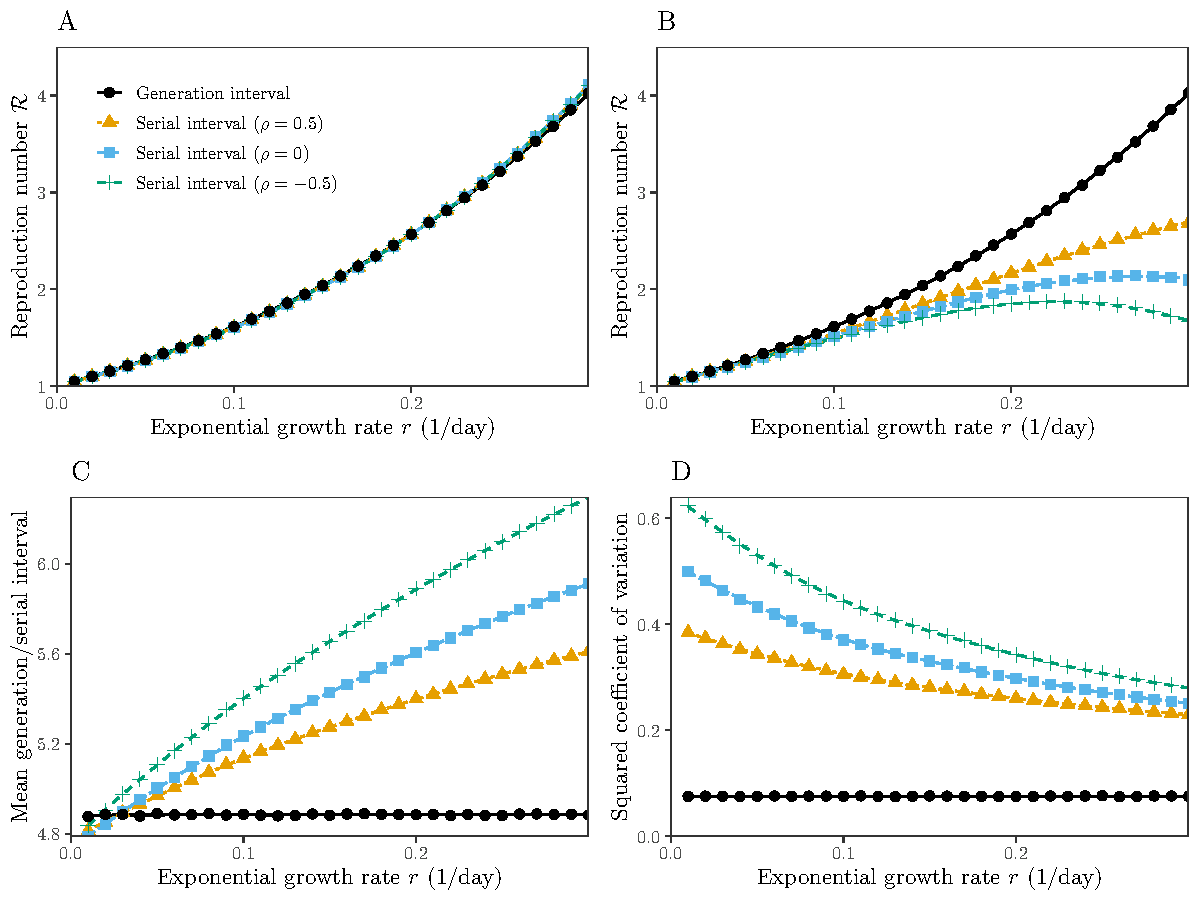
\includegraphics[width=\textwidth]{rR.pdf}
\caption{
\textbf{Estimates of the reproduction number from the exponential growth rate based on serial- and generation-interval distributions.}
(A). The initial forward serial-interval distributions give a correct link between the exponential growth rate $r$ and the reproduction number \Ro.
(B) The intrinsic serial-interval distributions give an incorrect link between $r$ and \Ro.
(C) The mean initial forward serial interval during the exponential growth phase depends on $r$.
(D) The squared coefficient of variation of the initial forward serial intervals during the exponential growth phase depends on $r$.
}
\label{fig:rR}
\end{figure}

Comparing the shapes of initial forward serial-interval distributions and the intrinsic generation-interval distribution allows us to better understand how different distributions are able to give identical estimates of \Ro.
In general, generation-interval distributions with higher means and less variability are expected to give higher \Ro for a given $r$ \citep{wallinga2007generation, park2019practical}.
In this case, the initial forward serial intervals during the exponential growth phase have higher means (\fref{rR}C) and squared coefficients of variation (\fref{rR}D) than the intrinsic generation-interval distribution.
The effects of higher means (which increases \Ro) and higher variability (which decreases \Ro) cancel out exactly;
this allows us to estimate the same \Ro using both initial forward serial and intrinsic generation intervals.
On the other hand, intrinsic serial intervals have the same mean (equal to the mean initial forward serial at $r=0$ in \fref{rR}C) as the intrinsic generation intervals but are wider (also see squared coefficient of variation of the initial forward serials at $r=0$ in \fref{rR}D); 
therefore, we underestimate \Ro when we use the intrinsic serial-interval distribution.

\begin{figure}[!ht]
\begin{center}
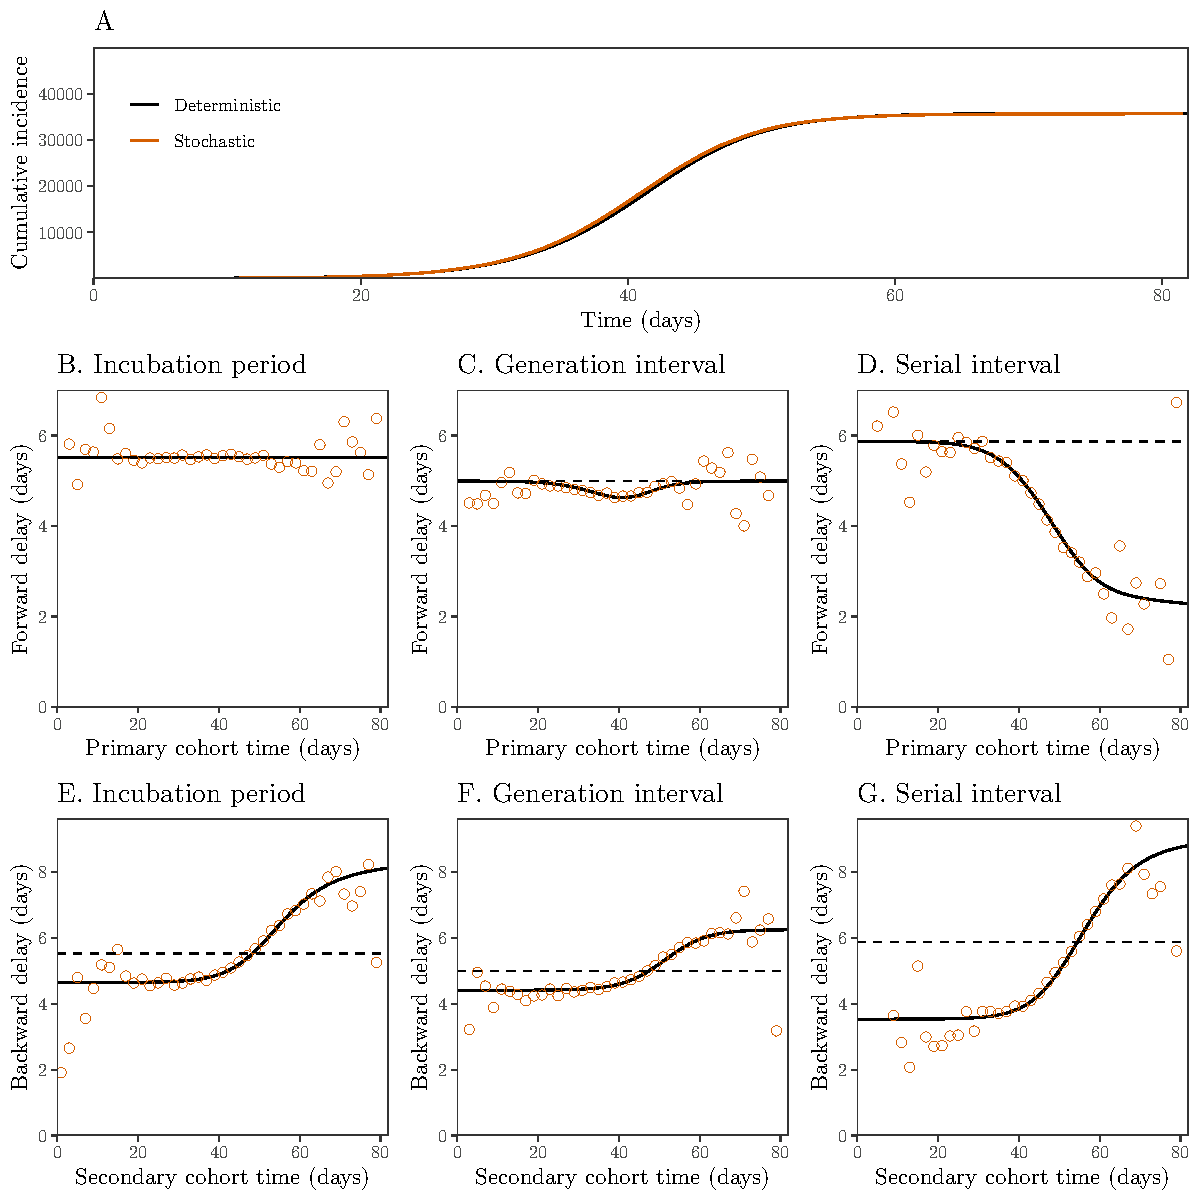
\includegraphics[width=0.95\textwidth]{forward.pdf}
\caption{
\textbf{Epidemiological dynamics and changes in mean forward and backward delay distributions.}
(A) Cumulative incidence over time.
(B--D) Changes in the mean forward incubation period, generation interval, and serial interval.
(E--G) Changes in the mean backward incubation period, generation interval, and serial interval.
Black lines represent the results of a deterministic simulation.
Orange lines and points represent the average of 10 stochastic simulations;
cumulative incidence from the stochastic simulations in panel A are shown without averaging.
Forward incubation periods and intrinsic generation-intervals are assumed to be independent of each other.
See Table 1 for parameter values.
}
\label{fig:epi}
\end{center}
\end{figure}

The initial forward serial interval distribution captures the exponential growth phase of an epidemic.
Now, we characterize how forward and backward serial intervals vary over the course of an epidemic when incubation periods and generation intervals are independent.
\fref{epi} compares the epidemiological dynamics (A) with the mean forward (B--D) and the mean backward (E--F) delay distributions of a deterministic model based on the renewal equation (\eref{renewal}) and of the corresponding stochastic realizations based on individual-based simulations.
The mean forward incubation period remains constant throughout an epidemic as assumed (\fref{epi}B).
The mean forward generation interval decreases slightly as incidence rate increases, causing the proportion of susceptible populaton to decrease (\fref{epi}C; \cite{kenah2008generation, champredon2015intrinsic}).
In contrast, the mean forward serial interval decreases over time (\fref{epi}D).

The forward serial interval distributions depend on three intervals (\fref{diagram}): (i) the backward incubation period distributions, (ii) the forward generation-interval distributions, and (iii) the forward incubation period distributions.
Since both forward incubation period (\fref{epi}B) and generation-interval (\fref{epi}C) distributions remain roughly constant, changes in the forward serial-interval distributions are predominantly driven by changes in the backward incubation period distributions, whose mean increases over time (\fref{epi}D). 
In this case, the increase in the mean backward incubation period directly translates to the decrease in the mean forward serial interval.
Therefore, the forward serial intervals can decrease over time even in the absence of significant depletion of the susceptible pool;
decrease in incidence via intervention strategies can still cause the backward incubation period to increase, which in turn can decrease serial intervals. 
In general, relative contributions of the three distributions depend on their shapes, correlations between incubation periods and generation intervals, and overall epidemiological dynamics.

Qualitative patterns in the mean backward delays is robust across all delay distributions because they are predominantly driven by the changes in incidence, which in turn affects cohort sizes (\fref{epi}D--F; \eref{backward}).
When incidence increases exponentially, individuals are more likely to have been infected more recently and therefore, we are more likely to observe shorter intervals (\eref{backexp}).
When incidence decreases, we are more likely to observe longer intervals for similar but opposite reasons.

\subsection{Observed serial interval distributions}

\begin{figure}[!ht]
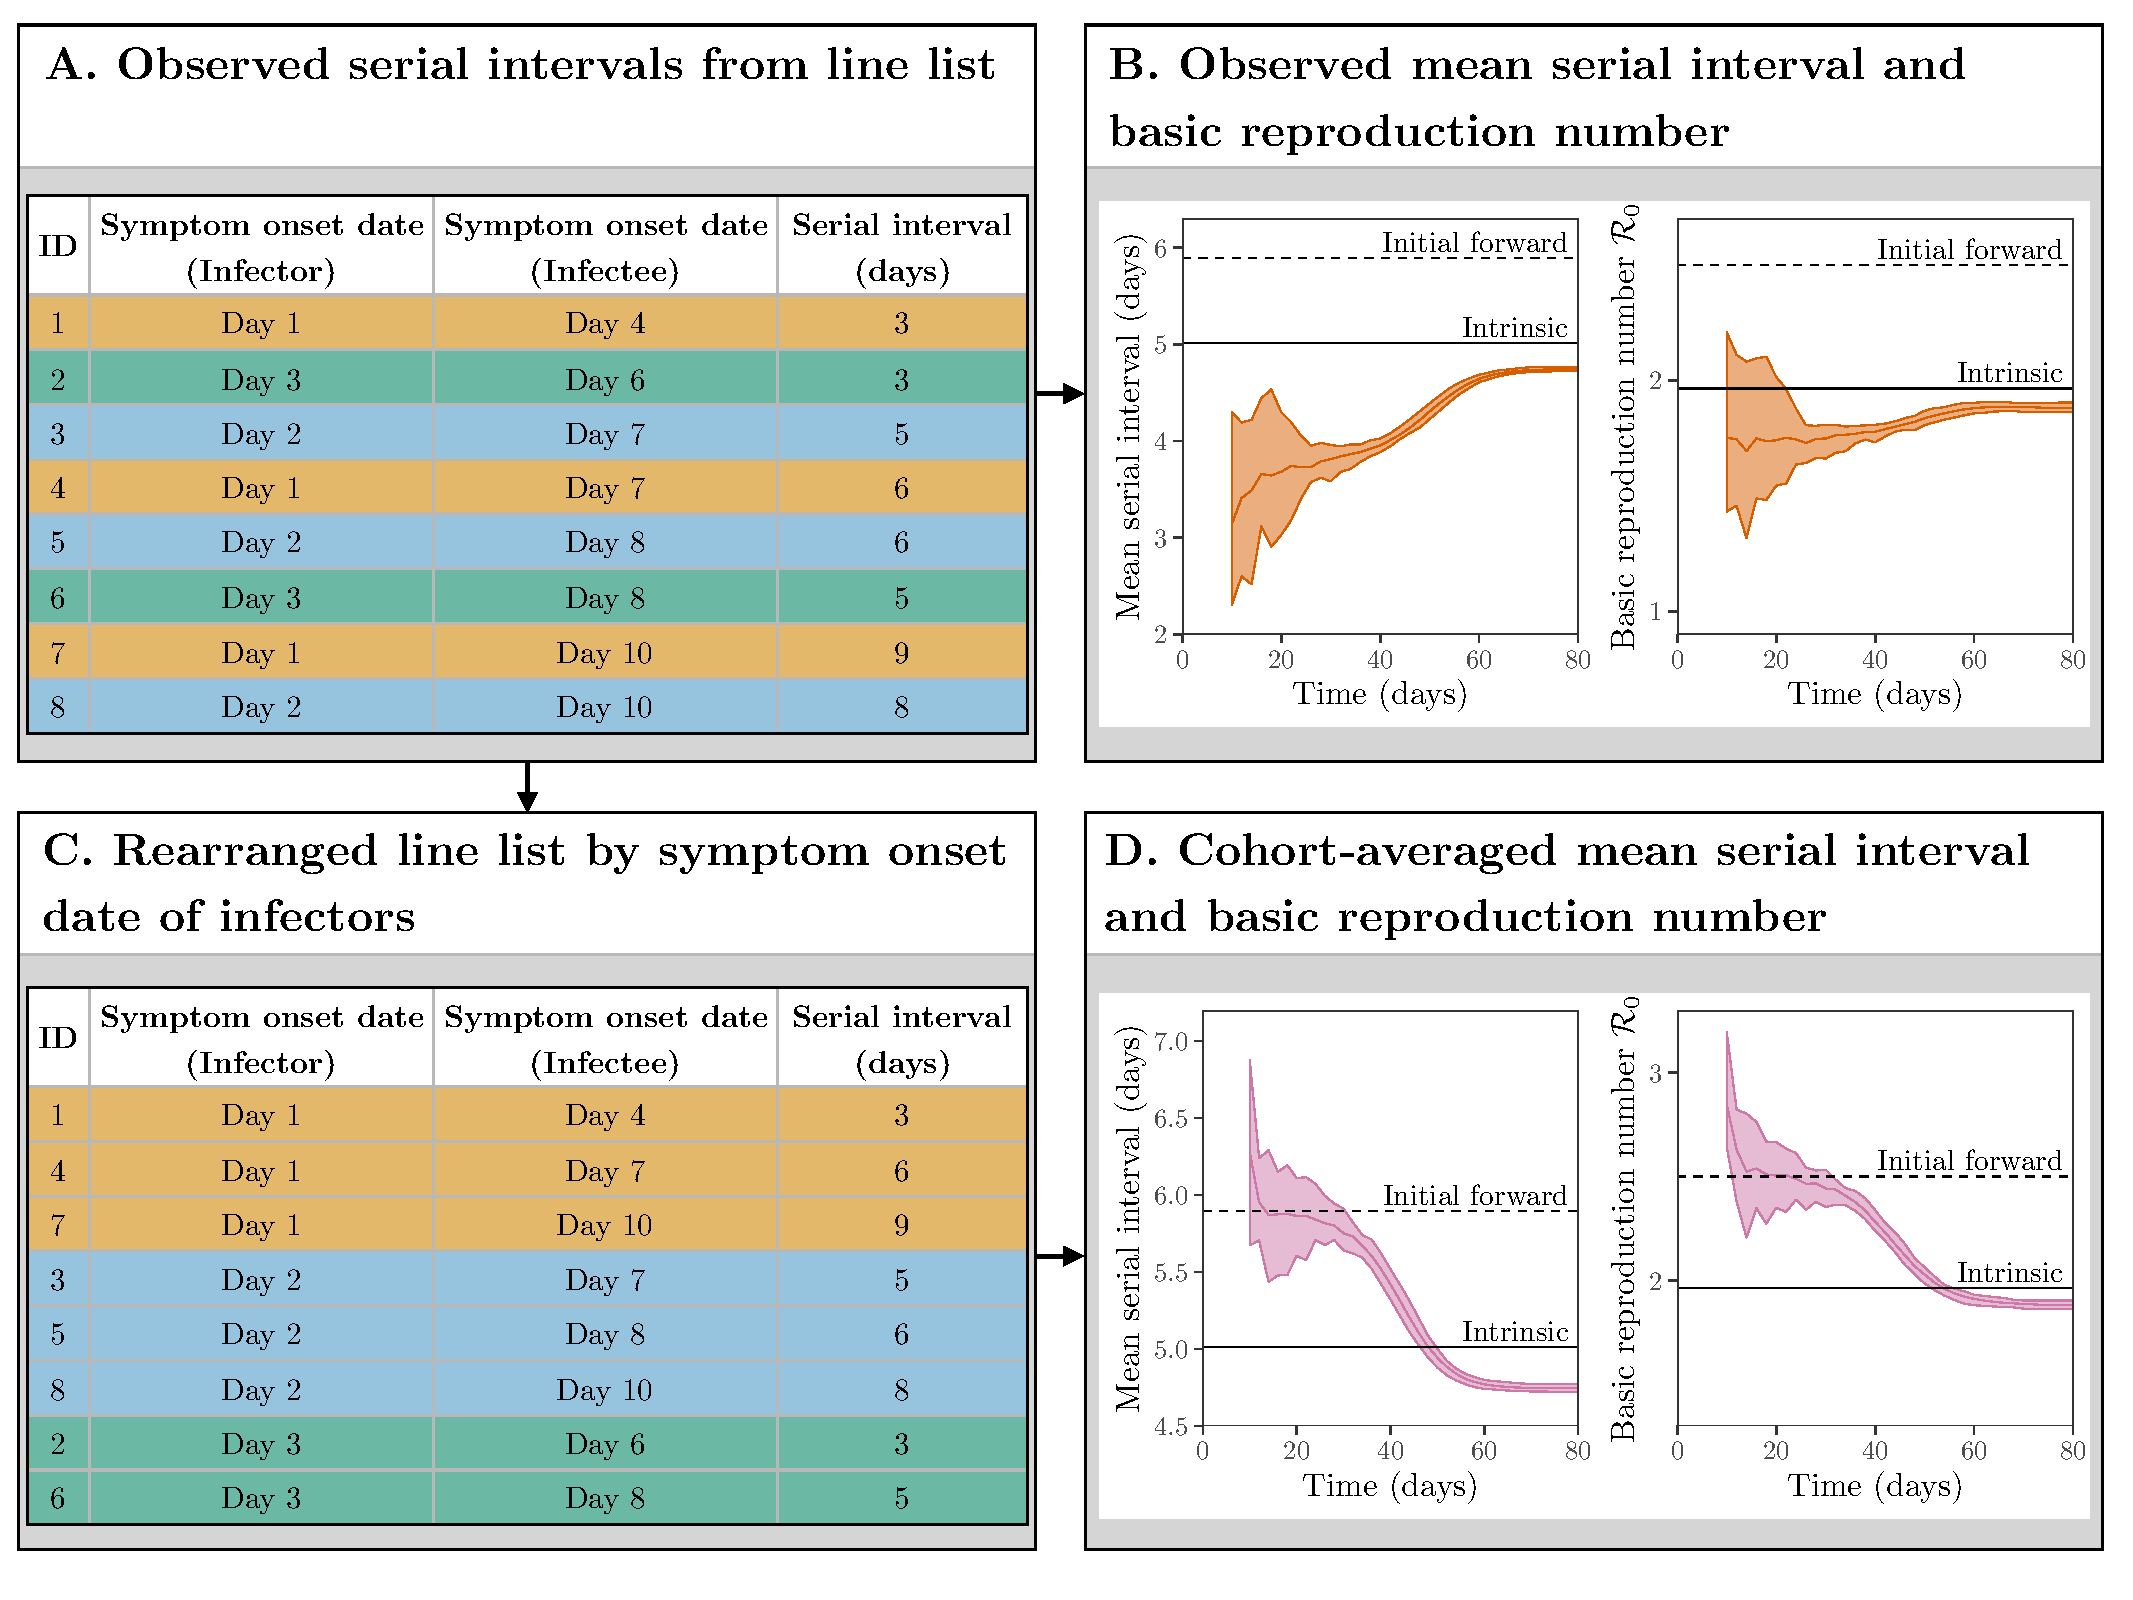
\includegraphics[width=\textwidth]{diagram.pdf}
\caption{
\textbf{Estimating the reproduction number from the observed serial intervals.}
(A) Schematic representation of line list data collected during an epidemic.
(B) Changes in the estimate of \Ro based on the observed serial intervals over time.
(C) Schematic representation of line list data rearranged by symptom onset date of infectors.
(B) Changes in the estimate of \Ro based on the cohort-averaged serial intervals over time.
Black dashed lines represent the mean initial forward serial interval and \Ro.
Black solid lines represent the mean intrinsic serial interval and \Rintrinsic.
Colored solid lines represent the mean estimates of \Ro across 10 stochastic simulations.
Colored ribbons represent the range of estimates of \Ro across 10 stochastic simulations.
}
\label{fig:obsrR}
\end{figure}

Now, we turn to practical issues.
In order to have an unbiased estimate on \Ro, we need to use serial-interval distributions estimated based on primary cohorts (i.e., infectors who share the same symptom onset time) at the early stage of the epidemic (i.e. initial forward serial-interval distribution).
However, when an epidemic is ongoing, the observed serial intervals are subject to right-censoring because we cannot observe a serial interval if either an infector or an infectee has not yet developed symptoms;
for example, if we were to measure serial intervals on Day 8 as in \fref{obsrR}A, we will only be able to observe the first 6 events (ID 1--6).
\fref{obsrR}B demonstrates how the effect of right-censoring in the observed serial intervals translates to the underestimation of the basic reproduction number \Ro in our stochastic simulations.
Notably, even if we can observe \emph{all} serial intervals across all transmission pairs after the epidemic has ended, we still underestimate the initial mean forward serial interval and therefore \Ro by a large amount because the observed serial-interval distribution converges to the intrinsic serial-interval distribution;
we still underestimate the intrinsic value slightly due to contraction of the forward generation-interval distribution during the susceptible depletion phase (\fref{epi}C).

We provide a simple, heuristic way of assessing potential biases in the estimate of the mean initial forward serial interval and therefore \Ro retrospectively.
Once serial intervals have been observed after the epidemic has been sufficiently progressed, we can rearrange the line list and group observed serial intervals based on the symptom onset date of infectors (\fref{obsrR}C).
Then, we can compare how estimates of the mean serial interval as well as \Ro change as we incorporate more recent cohorts into the analysis;
that is, we analyze observed serial intervals from infectors who became symptomatic before time $t$ and evaluate how the estimates change as we increase $t$
(\fref{obsrR}D).
During the exponential growth phase, the estimates of the mean serial interval and \Ro are consistent with the target value;
adding more data allows us to make more precise inference during this period.
However, the cohort-averaged estimates decrease rapidly soon after the exponential growth period, reflecting changes in the forward serial-interval distributions.
This approach allows us to detect dynamical changes in the forward serial-interval distributions and its effect on the estimates of \Ro.

\begin{figure}[!th]
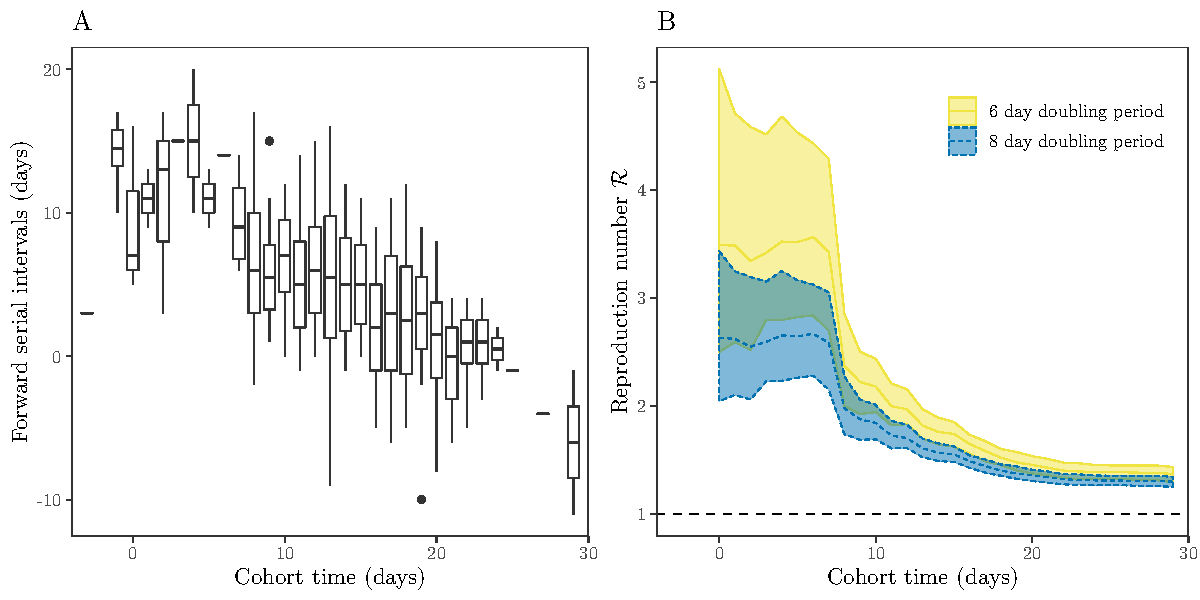
\includegraphics[width=\textwidth]{serial_analysis.pdf}
\caption{
\textbf{Observed serial intervals of COVID-19 and cohort-averaged estimates of \RR.}
(A--B) forward and backward serial intervals over time.
Points represent the means. 
Vertical error bars represent the 95\% equi-tailed quantiles.
Solid lines represent the estimated locally estimated scatterplot smoothing (LOESS) fits.
The dashed line represents the maximum observable delay for each primary cohort calculated from the most recent observed symptom onset date.
(C) Cohort-averaged estimates of \Ro assuming doubling period of 6 and 8 days \citep{li2020early, wu2020nowcasting}.
Ribbons represent the associated 95\% bootstrap confidence intervals.
The data were taken from Supplementary Materials of \cite{du2020serial}.
}
\label{fig:du}
\end{figure}

\subsection{Applications to the COVID-19 pandemic}

Finally, we re-analyze serial intervals of COVID-19 collected by \cite{du2020serial} from mainland China, outside Hubei province, based on transmission events reported between January 21--February 8, 2020;
\cite{du2020serial} estimated the mean serial of 3.96 days (95\% CI 3.53–4.39 days) and \Ro of 1.32 (95\% CI 1.16–1.48).
\fref{du}A shows that the mean forward serial interval decreases over time.
While the decrease is likely to be affected by the right-censoring (indicated by the closeness between the quantiles of the observed serial intervals and maximum \emph{observable} serial intervals), increase in the proportion of negative serial intervals are clearly indicative of the changes in the forward serial-interval distribution.
The decrease in the mean forward serial interval is likely to be cause by increase in the mean backward serial intervals as well as intervention efforts (e.g., case isolation will shorten the forward generation intervals).
\fref{du}B shows that the mean backward serial interval increases over time, reflecting decrease in incidence over time.

While the qualitative changes in the mean forward and backward serial interval are consistent with our earlier simulations (\fref{epi}), the initial mean forward serial interval (\fref{du}A) appears to be larger than what we calculate earlier based on previously estimated incubation period and generation-interval distributions (\fref{rR}C).
These results indicate that previous estimates of incubation period and generation-intervals may have been underestimated as neither study explicitly accounts for right-censoring (Table 1).

\fref{du}C shows the cohort-averaged estimates of \Ro, which remain roughly constant until day 7 and suddenly decreases;
this sudden decrease is indicative of changes in the forward serial intervals as shown in our simulation study (\fref{obsrR}).
The estimates of \Ro based on the early forward serial intervals are also consistent with previous estimates of \Ro of the COVID-19 epidemic in China \citep{majumder2020early, park2020reconciling}.
We note that early cohort-averaged estimates of \Ro are unlikely to be affected by the right-censoring as we expect the degree of right-censoring to be low (\fref{du}A).
This example clearly demonstrates the danger of using the observed serial intervals to calculate the basic reproduction number without integrating serial intervals into cohorts..

\section{Discussion}

Characterizing generation- and serial-interval distributions is critical to understanding the course of an outbreak as they determine the time scale of disease transmission.
Here, we show that the initial forward serial-interval distributions --- measured during exponential growth phase of an epidemic --- provides the correct link between the exponential growth rate $r$ and the reproduction number \RR.
We further illustrate that epidemiological dynamics can cause the mean backward incubation period to increase over time, which in turn decreases the mean forward serial interval.
Failing to account for these changes can result in underestimation of \RR.

Our study demonstrates the importance of defining a reference cohort for characterizing any epidemiological time distributions.
Previous studies have shown that generation interval can be either measured forward or backward \citep{nishiura2010time,champredon2015intrinsic,britton2019estimation};
we generalize their ideas and show that they can be applied to any distributions.
Changes in the backward delay distributions is expected to be a robust feature across any outbreaks because they are primarily driven by changes in cohort sizes, which, in turn, depend on incidence of infection.
Recent analyses of COVID-19 epidemics have attempted to reconstruct epidemic time series of symptomatic cases or infected cases from the reports of confirmed cases by using time-independent delay distributions from infection or symptom onset to reporting (e.g., \cite{tempvar, park2020potential, shim2020transmission});
these studies effectively assume constant backward delay distributions.
Although such approaches may be able to roughly match the time scale of an epidemic, we recommend using deconvolution approaches \citep{goldstein2009reconstructing} or mechanstic modeling approaches for proper reconstruction of epidemic time series instead \citep{flaxman2020estimating}.

Using cohort-based approaches, we define forward and backward serial intervals.
The forward serial-interval distribution describes the renewal process between symptomatic cases, and therefore, its initial distribution provides the correct link between $r$ and \RR.
While our results support the use of serial interval distributions for calculating \RR, 
they also reveal gaps in current practices in incorporating serial-interval distributions into outbreak analyses.
In particular, \cite{thompson2019improved} recently emphasized the importance of using up-to-date serial interval data for accurate estimation of time-varying reproduction numbers;
however, our study demonstrates that early serial interval data is required to estimate \RR and using up-to-date serial interval data can, in fact, underestaimte \RR.
Moreover, \cite{tempvar} recently analyzed case reports of COVID-19 from over 30 countries to estimate their time-varying reproduction numbers but relied on a serial-interval distribution;
given large geographical differences in the observed exponential growth rates of the COVID-19 epidemic, the initial forward serial interval distributions is likely to vary across different countries.
We suggest that modelers should aim to characterize spatiotemporal variation in initial forward serial-interval distributions and understand their changes over time.
These modeling approaches should be necessarily coupled with intensive epidemiological investigation through contact tracing at the very beginning of the outbreak in order to characterize the initial forward serial-interval distribution, particularly for an emerging epidemic such as COVID-19.

Our study also demonstrates that there are multiple serial-interval distributions that correspond to the same set of generation-interval and incubation period distributions depending on their correlations;
all of them can provide the correct link between $r$--\RR (\fref{rR}).
Conversely, this means that not explicitly accounting for their correlations can bias the estimate of the intrinsic generation-interval distribution from the serial-interval distribution.
Furthermore, previous studies that tried to estimate the generation-interval distributions from the observed serial intervals often ignored the differences between the incubation periods of infectors and those of infectees (e.g., \cite{klinkenberg2011correlation, ganyani2020estimating});
There is currently a need for better statistical tools for teasing apart the intrinsic generation-interval distributions from the observed serial intervals.

Our study is not without limitations.
Here, we assumed that all individuals develop symptoms and that the the entire transmission process (e.g., direction of transmission, symptom onset dates, infection dates, etc.) are observable.
In practice, asymptomatic and presymptomatic transmission of COVID-19 makes measuring serial intervals difficult \citep{bai2020presumed,he2020temporal,wei2020presymptomatic}.
For example, symptom onset dates cannot be used as a reliable proxy for determining the direction of transmission as infectees may develop symptoms before their infectors.
Based on the COVID-19 parameters (Table 1), we expect roughly 3\% of infectees to develop symptoms before their infectors during the exponential growth period; 
this probability increases as epidemic progresses because the mean backward incubation period increases.
Biases in the observed serial intervals will necessarily bias the estimates of \RR. 
Furthermore, serial intervals do not take into account asymptomatic transmission; 
not explicitly accounting for asymptomatic transmission may also bias the estimates of \RR \citep{park2020time}.

While we focused on the effect of epidemiological dynamics on the serial-interval distributions, other factors, such as intervention strategies, can also affect the generation- and serial-interval distributions.
Individual-level interventions, such as case isolation, directly affect individual's ability to transmit and will shorten the forward generation- and serial-intervals.
On the other hand, population-level interventions, such as social distancing, have qualitatively similar effects on epidemiogical dynamics as susceptible depletion;
therefore, we expect these intervention efforts to also shorten the forward generation- and serial-intervals.

Despite these limitations, our analysis of serial intervals of COVID-19 from China provide further support for our theoretical framework, demonstrating temporal variation in serial intervals and their effects on the estimates of \RR.
To our knowledge, most existing estimates of the serial-intervals of COVID-19 implicitly or explicitly assume that the serial-interval distributions remain constant throughout the course of an epidemic \citep{du2020serial, he2020temporal, nishiura2020serial,tindale2020transmission,zhao2020estimating,zhang2020evolving}.
Our study provides a rationale for reassessing estimates of serial-interval distributions, and their use in estimating \Ro, of the COVID-19 pandemic.

\pagebreak

\section{Appendix}

\subsection{Deterministic simulation}

We simulate the renewal equation model using a discrete-time approximation:
\begin{equation}
\begin{aligned}
i(t) &= \Ro S(t-\Delta t) \sum_{m=1}^{\ell} i(t-m \Delta t) \hat{\gdist}(m \Delta t) \\
S(t) &= S(t-\Delta t) - i(t)
\end{aligned}
\end{equation}
where $\hat{\gdist}$ is a discrete-time intrinsic generation-interval distribution that satisfies the following:
\begin{equation}
\hat{\gdist}(m \Delta t) = \frac{\gdist(m \Delta t)}{\sum_{i=1}^\ell \gdist(m \Delta t)}, \quad m=1, \dots, \ell
\end{equation}
The continuous-time intrinsic generation-interval distribution is parameterized using a log-normal distribution (Table 1). We define the forward incubation period distribution in a similar manner:
\begin{equation}
\hat{k}(m \Delta t) = \frac{k(m \Delta t)}{\sum_{i=1}^\ell k(m \Delta t)}, \quad m=1, \dots, \ell,
\end{equation}
where its continuous-time analog is also based on a log-normal distribution.
For brevity, we assume that the forward incubation periods and intrinsic generation intervals are independent:
\begin{equation}
\hat{h}(m \Delta t, \Delta t n) = \hat{k}(m \Delta t)\hat{\gdist}(\Delta t n), \quad m,n=1, \dots, \ell.
\end{equation}
We use $\Delta t = 0.025\,\textrm{days}$ and $\ell=2001$ for discretization steps.

We initialize the simulation with population size $N$=40,000 as follows:
\begin{equation}
\begin{aligned}
i(m \Delta t) &= C \exp(r m \Delta t), \quad m=1, \dots, \ell\\
S(m \Delta t) &= N - \sum_{n=1}^m i(m \Delta t), \quad m=1, \dots, \ell\\
\end{aligned}
\end{equation}
where $C$ is chosen such that $\sum_{n=1}^\ell i(m \Delta t)=10$.
These initial conditions allow the model to follow exponentially growth from time $\Delta t (\ell + 1)$ without any transient behaviors.
Results presented in the main text show simulations beginning from time $\Delta t (\ell + 1)$.

\subsection{Stochastic simulation}

We run stochastic simulations of the renewal equation model using an individual-based model on a fully connected network (i.e., homogeneous population) based on the Gillespie algorithm that we developed earlier \citep{park2019inferring}.
First, we initialize an epidemic with $I(0)$ infected individuals (nodes) in a fully connected network of size $N$. 
For each initially infected individual, we draw number of infectious contacts from a Poisson distribution with the mean of \Ro and the corresponding generation intervals for each contact from a log-normal distribution (Table 1).
Contactees are uniformly sampled from the total population.
All contactees are sorted into event queues based on their infection time.
We update the current time to the infection time of the first person in the queue.
Then, the first person in the queue makes contacts based on the Poisson offspring distribution described earlier and their contactees are added to the sorted queue.
Whenever contactees are added to the sorted queue, we remove all duplicated contacts (but keep the first one) as well as contacts made to individuals that have already been infected.
Simulations continue until there are no more individuals in the queue.
We simulate 10 epidemics with $I(0)=10$ and $N$=40,000.

\subsection{Linking $r$ and \RR using serial-interval distributions}

The intrinsic generation-interval distribution $\gdist(\tau)$ provides a link between $r$ and \Ro via the Euler-Lotka equation:
\begin{equation}
\frac{1}{\Ro} = \int_0^\infty \exp(-r\tau) \gdist(\tau) \dtau.
\end{equation}
Here, we prove that the initial forward serial-interval distribution $f_0$ also provides the same link:
\begin{equation}
\frac{1}{\Ro} = \int_{-\infty}^\infty \exp(-r\tau) f_{0}(\tau) \dtau,
\end{equation}
where the initial forward serial-interval distribution is defined as:
\begin{equation}
f_{0}(\tau) \propto \int_{0}^{\infty} \int_{0}^{\max(0,x+\tau)} \exp(-rx) h(x, \sigma) k(x-\sigma+\tau) \dsigma\dx.
\end{equation}

First, we rewrite the initial forward serial-interval distribution in the following form:
\begin{equation}
\begin{aligned}
f_{0}(\tau) &\propto \int_0^\infty \int_{-\alpha_1}^{\tau} \exp(-r\alpha_1) h(\alpha_1, \alpha_2 + \alpha_1) k(\tau - \alpha_2) \mathrm{d}\alpha_2\,\mathrm{d}\alpha_1\\
&= \int_{-\infty}^{\tau} \int_{\max{(0,-\alpha_2)}}^{\infty} \exp(-r\alpha_1) h(\alpha_1, \alpha_2 + \alpha_1)k(\tau - \alpha_2)\mathrm{d}\alpha_1\, \mathrm{d}\alpha_2\\
\end{aligned}
\end{equation}
It follows that $z(\alpha_2)$ describes the time between symptom onset of infector and infection of infectee:
\begin{equation}
z(\alpha_2) \propto \int_{\max{(0,-\alpha_2)}}^{\infty} \exp(-r\alpha_1) h(\alpha_1, \alpha_2 + \alpha_1) \mathrm{d}\alpha_1.
\end{equation}
The initial forward serial-interval distribution $f_0$ can be expressed as a convolution of $z$ and $k$:
\begin{equation}
\begin{aligned}
f_{0}(\tau) &\propto \int_{-\infty}^{\tau} z(\alpha_2) k(\tau - \alpha_2) \mathrm{d}\alpha_2.\\
\end{aligned}
\end{equation}
Then, we have
\begin{equation}
\int_{-\infty}^\infty \exp(-r\tau) f_{0}(\tau) \mathrm{d} \tau = \int_{-\infty}^\infty \exp(-r\tau) z(\tau) \mathrm{d} \tau \int_{0}^\infty \exp(-r\tau) k(\tau) \mathrm{d} \tau
\end{equation}

Note that 
\begin{equation}
\begin{aligned}
&\int_{-\infty}^\infty \int_{\max{(0,-\alpha_2)}}^{\infty} \exp(-r\alpha_1) h(\alpha_1, \alpha_2 + \alpha_1) \mathrm{d}\alpha_1 \mathrm{d}\alpha_2\\
&= \int_{0}^\infty \int_{-\alpha_1}^\infty \exp(- r \alpha_1) h(\alpha_1, \alpha_2+\alpha_1) \mathrm{d}\alpha_2\,\mathrm{d} \alpha_1\\
&= \int_{0}^\infty \exp(- r \alpha_1) k(\alpha_1) d\alpha_1
\end{aligned}
\end{equation}
because $k$ is a marginal probability distribution of $h$.
Since $\int_{0}^\infty \exp(- r \alpha_1) k(\alpha_1) d\alpha_1$ is a normalization factor for probability distribution $z$, we have:
\begin{equation}
\int_{-\infty}^\infty \exp(-r\tau) z(\tau) \mathrm{d} \tau = \frac{\int_{-\infty}^\infty \exp(-r\tau) \int_{\max{(0,-\alpha_2)}}^{\infty} \exp(-r\alpha_1) h(\alpha_1, \alpha_2 + \alpha_1) \mathrm{d}\alpha_1 \mathrm{d}\tau}{\int_{0}^\infty \exp(- r \alpha_1) k(\alpha_1) d\alpha_1}.
\end{equation}
Then, we have:
\begin{equation}
\int_{-\infty}^\infty \exp(-r\tau) f_{0}(\tau) \mathrm{d} \tau = \int_{-\infty}^\infty \exp(-r\tau) \int_{\max{(0,-\alpha_2)}}^{\infty} \exp(-r\alpha_1) h(\alpha_1, \alpha_2 + \alpha_1) \mathrm{d}\alpha_1 \mathrm{d}\tau.
\end{equation}

We are left to show that 
\begin{equation}
\int_0^{\infty} \exp(-r\tau) g(\tau) \mathrm{d}\tau = \int_{-\infty}^\infty \exp(-r\tau) \int_{\max{(0,-\alpha_2)}}^{\infty} \exp(-r\alpha_1) h(\alpha_1, \alpha_2 + \alpha_1) \mathrm{d}\alpha_1 \mathrm{d}\tau,
\end{equation}
where the intrinsic generation-interval distribution $g$ is also a marginal probability distribution of $f$:
\begin{equation}
g(\tau) = \int_0^\infty h(\alpha_1, \tau)  \mathrm{d} \alpha_1.
\end{equation}
Let $\sigma = \alpha_1 + \tau$. Then, by change of variables, it immediately follows that
\begin{equation}
\begin{aligned}
&\int_{-\infty}^{\infty} \exp(-r\tau) \int_{\max(0, -\tau)}^\infty \exp(- r \alpha_1) h(\alpha_1, \tau+\alpha_1) \mathrm{d} \alpha_1\, \mathrm{d}\tau\\
&=\int_{0}^{\infty} \int_{0}^\infty \exp(- r \sigma) h(\alpha_1, \sigma) \mathrm{d} \alpha_1\, \mathrm{d}\sigma\\
&=\int_{0}^{\infty} \exp(-r\tau) g(\tau) \mathrm{d}\tau
\end{aligned}
\end{equation}
Therefore, the initial forward serial--interval distribution and the intrinsic generation-interval distribution give the same link between $r$ and \RR.

\bibliography{serial}

\end{document}
